\documentclass[tikz]{standalone}

% Copy of relevant parts from the main preamble.
\usepackage{mathtools}

% Uncomment the following to use Times New Roman and Cambria Math
% \usepackage{unicode-math}
% \unimathsetup{math-style=TeX}
% \setmathfont[range=\mathup/{num}]{Times New Roman}
% \setmathfont[range=\mathit/{greek,Greek,latin,Latin}]{Cambria Math}
% \setmathfont[range=\mathup/{greek,Greek,latin,Latin}]{Cambria Math}
% \setmathfont[range={"2212,"002B,"003D,"0028,"0029,"005B,"005D,"221A,
% "2211,"2248,"222B,"007C,"2026,"2202,"00D7,"0302,"2261,"0025,"22C5,
% "00B1,"2194,"21D4,"2032}]
% {Cambria Math}
% \setmainfont[Ligatures=TeX]{Times New Roman}

% Uncomment the following to use Linux Libertine
% \usepackage[libertine]{newtxmath}
% \usepackage[no-math]{fontspec}
% \setmainfont{Linux Libertine O}

% Uncomment the following to use TeX Gyre Termes
% \usepackage{unicode-math}
% \unimathsetup{math-style=TeX}
% \setmainfont{TeX Gyre Termes}
% \setmathfont{TeX Gyre Termes Math}

% Uncomment the following to use TeX Gyre Pagella
\usepackage{unicode-math}
\unimathsetup{math-style=TeX}
\setmainfont{TeX Gyre Pagella}
\setmathfont{TeX Gyre Pagella Math}

% \usepackage[sfmath]{kpfonts}
% \renewcommand*\familydefault{\sfdefault}
% \usepackage[T1]{fontenc}

% \usepackage[no-math]{fontspec}
% Always use Inconsolata
\setmonofont{Inconsolata}

\usepackage{microtype}


\usetikzlibrary{patterns, positioning, arrows.meta}

\pgfdeclarepatternformonly[\LineSpace]{my north east lines}{\pgfqpoint{-1pt}{-1pt}}{\pgfpoint{\LineSpace}{\LineSpace}}{\pgfpoint{\LineSpace-0.5pt}{\LineSpace-0.5pt}}%
{
    \pgfsetlinewidth{0.4pt}
    \pgfpathmoveto{\pgfqpoint{0pt}{0pt}}
    \pgfpathlineto{\pgfpoint{\LineSpace}{\LineSpace}}
    \pgfusepath{stroke}
}

\pgfdeclarepatternformonly[\LineSpace]{my north west lines}{\pgfqpoint{-1pt}{-1pt}}{\pgfpoint{\LineSpace}{\LineSpace}}{\pgfpoint{\LineSpace-1pt}{\LineSpace-1pt}}%
{
    \pgfsetlinewidth{0.4pt}
    \pgfpathmoveto{\pgfpoint{0pt}{\LineSpace}}
    \pgfpathlineto{\pgfpoint{\LineSpace}{0pt}}
    \pgfusepath{stroke}
}

\newdimen\LineSpace
\tikzset{
    line space/.code={\LineSpace=#1},
    line space=3pt
}

\begin{document}
    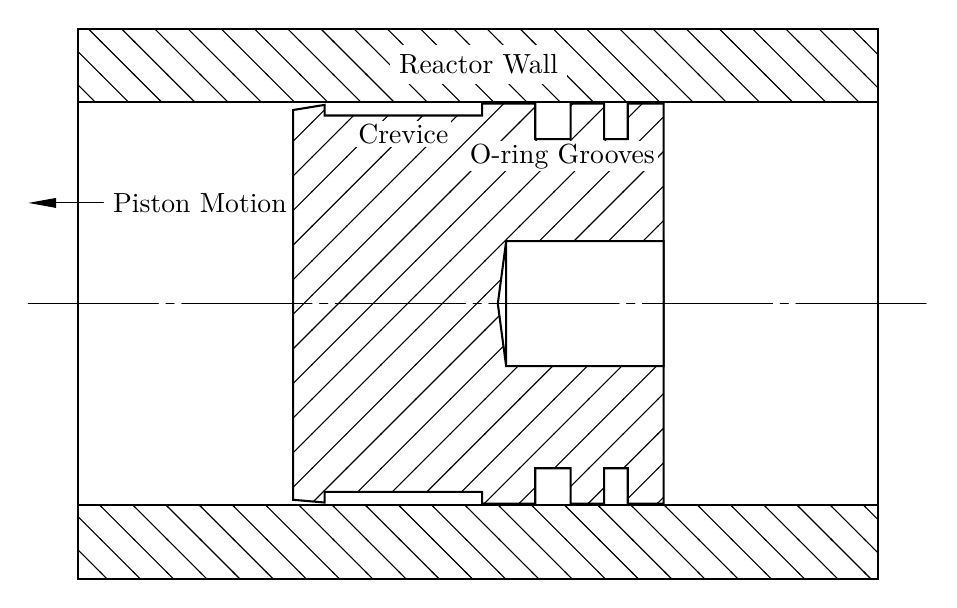
\begin{tikzpicture}
        \pgfmathsetlengthmacro{\reactorwidth}{4in}
        \pgfmathsetlengthmacro{\reactordia}{51.2mm}
        \pgfmathsetlengthmacro{\outerdia}{2.75in}
        \pgfmathsetlengthmacro{\pistondia}{50.8mm}
        \pgfmathsetlengthmacro{\pistonlength}{47.06mm}
        \pgfmathsetlengthmacro{\A}{0.50mm}
        \pgfmathsetlengthmacro{\B}{4.00mm}
        \pgfmathsetlengthmacro{\C}{0.15mm}
        \pgfmathsetlengthmacro{\D}{20.0mm}
        \pgfmathsetlengthmacro{\E}{1.50mm}
        \pgfmathsetlengthmacro{\oringdepth}{4.5mm}
        \pgfmathsetlengthmacro{\smalloringwidth}{3mm}
        \pgfmathsetlengthmacro{\bigoringwidth}{4.5mm}
        \pgfmathsetlengthmacro{\gaptofirstoring}{4.56mm}
        \pgfmathsetlengthmacro{\gaptosecoring}{4.25mm}
        \pgfmathsetlengthmacro{\gaptocrevice}{6.75mm}
        \pgfmathsetlengthmacro{\boltholedia}{0.625in}
        \pgfmathsetlengthmacro{\boltholelen}{20mm}
        \pgfmathsetlengthmacro{\boltcapheight}{1.06mm}

        \node[draw, line width=0.75pt, pattern=my north west lines, line space=13pt, minimum width=\reactorwidth, minimum height=\outerdia] (reactor wall) at (0,0) {};
        \node[draw, line width=0.75pt, fill=white, minimum width=\reactorwidth, minimum height=\reactordia] (reactor) at (0,0) {};
        \filldraw[line width=0.75pt, pattern=my north east lines, line space=13pt] (\pistonlength/2,\pistondia/2) -| ++(-\gaptofirstoring,-\oringdepth) -| ++(-\smalloringwidth,\oringdepth) -| ++(-\gaptosecoring,-\oringdepth) -| ++(-\bigoringwidth,\oringdepth) -- ++(-\gaptocrevice,0) -- ++(0,-\E) -- ++(-\D,0) coordinate[midway] (crevice) -- ++(0,\E-\C) -- ++(-\B,-\A-\C) -- ++(0,-\pistondia+2*\A+2*\C) -- ++(\B,-\A+\C) -- ++(0,\E-\C) -| ++(\D,-\E) -| ++(\gaptocrevice,\oringdepth) -| ++(\bigoringwidth,-\oringdepth) -| ++(\gaptosecoring,\oringdepth) -| ++(\smalloringwidth,-\oringdepth) -| ++(\gaptofirstoring,\pistondia) --cycle;
        \draw[fill=white, line width=0.75pt] (\pistonlength/2,\boltholedia/2) rectangle ++(-\boltholelen,-\boltholedia) -- ++(-\boltcapheight,\boltholedia/2) -- ++(\boltcapheight,\boltholedia/2);
        \draw[dash pattern=on 16.5mm off 1mm on 1mm off 1mm, line cap=round, line width=0.5pt] (-\reactorwidth/2-0.25in,0) -- (\reactorwidth/2+0.25in,0);
        \begin{scope}[x={(reactor.north east)},y={(reactor wall.north west)}]
            \node[fill=white] at (0.5,0.5) {Reactor Wall};
        \end{scope}
        \node[below=0 of crevice, fill=white, inner sep=1pt, outer sep=2pt] {Crevice};
        \node[below right=0.25 and 0.74 of crevice, fill=white, inner sep=1pt, outer sep=2pt] {O-ring Grooves};
        \draw[{Triangle[length=10pt, width=3.5pt]}-, line cap=round] (-\reactorwidth/2-0.25in,\reactordia/4) -- ++(0.375in,0) node[anchor=west] {Piston Motion};
    \end{tikzpicture}
\end{document}